Os modelos propostos e seus respectivos parâmetros e hiperparâmetros para a tarefa de classificação de expressões faciais são descritos detalhadamente ao longo desta seção.

Seguindo a abordagem predominantemente adotada pelo estado da arte no tocante ao aprendizado de características em dados de alta dimensionalidade para tarefas de Visão Computacional \cite{Khan:Livro}, as redes neurais convolucionais foram o modelo de Aprendizado de Máquina adotado na tarefa elencada. Em particular, a arquitetura base foi a da rede neural convolucional canônica VGG-16 \cite{VGG}, mas com algumas adaptações. Esta arquietura originalmente proposta  destacou-se mediante a ideia de que uma rede neural precisa ter uma quantidade razoável  de camadas convolucionais profundas para uma representação hierárquica adequada das informações visuais.

As adaptações da VGG-16 levaram em conta diferentes quantidades de repetições de certas operações, apresentadas de acordo com a seguinte ideia geral:
\begin{equation}
\begin{split}
\textrm{Camada de Entrada} & \Rightarrow [ (\textrm{Convolução} \rightarrow \textrm{Batch Normalization})\cdot i\\
 &\quad \Rightarrow (\textrm{Pooling} \rightarrow \textrm{Dropout})\cdot j]\cdot k \\
 &\quad \Rightarrow [\textrm{Fully Connected} \rightarrow \textrm{ReLu}]\cdot \ell \\
 &\quad \Rightarrow \textrm{Flatten} \Rightarrow \textrm{Camada de Saída},
\end{split}
\end{equation} em que $i, j, k, \ell$ são números inteiros que denotam a quantidade de repetições da operação associada perante multiplicação. Os valores destes inteiros foram: $i = 2$, $j = \{1, \ldots, 5\}$, $k = \{2, 3, 4\}$ e $\ell = \{ 1,2,3 \}$.\ Considerando esta abordagem de adaptação, foram então propostas $9$ CNNs diferentes a serem treinadas e testadas, conforme a abordagem de validação cruzada previamente descrita.

% Complementar um pouco os parâmetros que você falou depois

Além da avaliação individual do desempenho das CNNs propostas, considerou-se também a posterior combinação destas redes em um \emph{ensemble}. Para valoração da classificação final, ao invés de considerar as abordagens típicas de votação unânime ou majoritária adotadas por \emph{ensembles}, utilizou-se um modelo baseado em \emph{Boosting}, o XGBoost \cite{Chen:Boosting}. Este modelo recebe as saídas de todas as redes individuais e, após ter sido treinado com os exemplos da base de dados, decide dentre as classificações individuais qual a classificação final mais apropriada. Observa-se aqui uma modificação não-trivial em \emph{ensembles}: a votação mediada por um modelo inteligente. A Figura X ilustra a ideia considerada.

\begin{figure}[!htb]
    \centering
    \caption{\emph{Ensemble} de CNNs com votação mediada por XGBoost.} \label{fig:ensemble}
    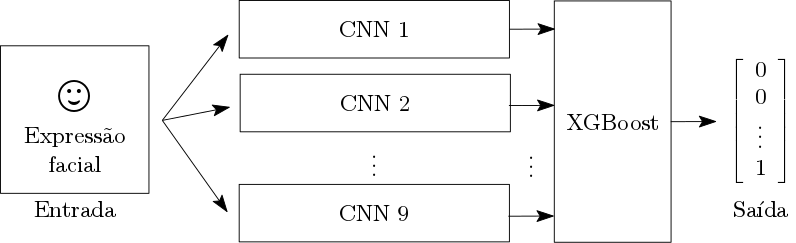
\includegraphics[width=0.9\textwidth]{images/ensemble-elloa.png}
\end{figure}



\iffalse
O modelo proposto consiste de um conjunto de \emph{Convolutional Neural Networks} (CNN), onde cada elemento é responsável pela classificação da imagem de entrada em uma das Sete Expressões Faciais Universais \cite{}, por meio da produção de vetor de probabilidades. Que consiste na possibilidade de cada uma das expressões universais estarem sendo expressas pela face, na imagem. A determinação da classificação final, não segue as abordagens típicas da literatura, via maioria ou consenso. Pois, estes vetores de probabilidades foram utilizados, de maneira supervisionada, para treinar um modelo do tipo \emph{XGBoost}, que finalmente atribui o rótulo mais adequado à entrada. Tem-se então um \emph{emsemble} de CNN com processo decisório de classificação realizado de maneira não trivial por um modelo de \emph{Machine Learning}.

O objetivo com a união de vários modelos de CNN foi obter classificadores bons de maneira geral em todas as expressões, contudo, estes deveriam se sobressair em determinadas expressões. Com isso, foram gerados sete modelos, um para cada expressão que deveriam ser classificadas, contudo, além dos sete classificadores bons individualmente na classificação de determinada expressão, adicionou-se dois outros, os quais obtiveram melhor desempenho considerando a classificação de todas as expressões, mas não obtiveram melhores resultados em determinada expressão em relação aos classificadores individuais.

Segundo \cite{}, o modelo \emph{XGBoost} é um bom modelo para se utilizar na técnica \emph{Boost}, que tem como objetivo obter um modelo \emph{Stronger} baseado nas combinações das respostas de \emph{Weak Learners}. Visto isso, foi considerado cada modelo de CNN, como um \emph{Weak Learner}, apesar de eles não serem fracos, dada a complexidade da tarefa e seus resultado, Tabela \ref{tbl:fscore}. E como saída estes forneciam seus resultados, vetores de probabilidade, para o modelo \emph{XGBoost} que tratava de melhor combinar os resultados individuais para se obter um melhor resultado de predição.

As arquiteturas CNN utilizadas na construção do modelo, foram baseadas na arquitetura \emph{VGG-16} \cite{}, que consiste de camadas duplas ou triplas de convolução 2D, com \emph{kernel} de 3x3, seguidas de \emph{pooling}, utilizando \emph{MaxPooling}. E como saída tem camadas densas, também chamadas de \emph{Fully Connected} (FC), onde a última utiliza a função de ativação \emph{SoftMax}.

Como função de ativação para as camadas convolucionais e densas, foi utilizada a função \emph{ReLU}, devido ao seu baixo custo computacional, e também possuir derivada constante, o que contribui para o desempenho da função de otimização \emph{adam} \cite{}. Segundo \cite{}, e análise experimental, a inicialização dos pesos iniciais das camadas convolucionais que utilizam a função de ativação \emph{ReLu}, com o inicializador de He et al \cite{}, possibilita aumento no desempenho, convergência, durante o treinamento dos modelos CNN.

Após a saída de cada camadas convolucionais, foi utilizada normalização em lotes, \emph{Batch Normalization}, pois, segundo \cite{} e análise experimental, os modelos modelos de CNN possuem melhores resultados nas predições, tanto na etapa de treinamento quanto na etapa de generalização.

Algumas das "regras de ouro" \cite{} para construção de modelos baseados em \emph{Artificial Neural Networks} (ANN) foram utilizadas nas camadas densas, visto que estas são equivalentes. Foram elas: A quantidade de neurônios das cadas ocultas não deve ultrapassar o dobro da quantidade dados da entrada, e a quantidade de neurônios da camada de entrada deve ser a mesma da quantidade de dados da entrada. Vale ressaltar, que as camadas de \emph{FC} em sua maioria não possuem mais do que duas camadas ocultas, devido ao Teorema de aproximação universal \cite{}.

Para regularização dos modelos de CNN foi utilizado somente \emph{Dropout}, visto que os regularizadores $l1$ e $l2$, não apresentaram bons resultados durante o período de treinamento, o que tornavam o modelo instável ou com tendências a \emph{underfitting}. Essa tendência foi evidenciada pelo desempenho constante do modelo por algumas dezenas de épocas de treinamento, e ao ser percebido esse comportamento o treinamento foi interrompido.

A arquitetura final dos modelos de CNN podem ser visualizados na Tabela \ref{tbl:arch}. Já a arquitetura utilizada pelo \emph{XGBoost} não pode ser mostrada, devido a esta ter mil árvores classificadoras, o que torna inviável a apresentação desta neste artigo.

\begin{table}
\centering
\caption{Arquiteturas utilizadas}
\label{tbl-arch}
\resizebox{\textwidth}{!}{%
\begin{tabular}{@{}lllllllll@{}}
\toprule
\multicolumn{1}{c}{1} & \multicolumn{1}{c}{2} & \multicolumn{1}{c}{3} & \multicolumn{1}{c}{4} & \multicolumn{1}{c}{5} & \multicolumn{1}{c}{6} & \multicolumn{1}{c}{7} & \multicolumn{1}{c}{8} & \multicolumn{1}{c}{9} \\ \midrule
Conv2D\_(64, 3, 3)    & Conv2D\_(64, 3, 3)    & Conv2D\_(64, 3, 3)    & Conv2D\_(64, 3, 3)    & Conv2D\_(64, 3, 3)    & Conv2D\_(64, 3, 3)    & Conv2D\_(128, 7, 7)   & Conv2D\_(16, 7, 7)    & Conv2D\_(16, 7, 7)    \\
BatchNorm             & BatchNorm             & BatchNorm             & BatchNorm             & BatchNorm             & BatchNorm             & BatchNorm             & BatchNorm             & BatchNorm             \\
Conv2D\_(64, 3, 3)    & Conv2D\_(64, 3, 3)    & Conv2D\_(64, 3, 3)    & Conv2D\_(64, 3, 3)    & Conv2D\_(64, 3, 3)    & Conv2D\_(64, 3, 3)    & Conv2D\_(128, 7, 7)   & Conv2D\_(16, 7, 7)    & Conv2D\_(16, 7, 7)    \\
BatchNorm             & BatchNorm             & BatchNorm             & BatchNorm             & BatchNorm             & BatchNorm             & BatchNorm             & BatchNorm             & BatchNorm             \\
MaxPool\_(3, 3)       & MaxPool\_(3, 3)       & MaxPool\_(3, 3)       & MaxPool\_(3, 3)       & MaxPool\_(3, 3)       & MaxPool\_(3, 3)       & AvgPool\_(3, 3)       & AvgPool\_(3, 3)       & AvgPool\_(3, 3)       \\
Dropout\_50           & Dropout\_50           & Dropout\_50           & Dropout\_50           & Dropout\_50           & Dropout\_50           & Dropout\_50           & Dropout\_50           & Dropout\_50           \\
Conv2D\_(128, 3, 3)   & Conv2D\_(128, 3, 3)   & Conv2D\_(128, 3, 3)   & Conv2D\_(128, 3, 3)   & Conv2D\_(128, 3, 3)   & Conv2D\_(128, 3, 3)   & Conv2D\_(128, 5, 5)   & Conv2D\_(32, 3, 3)    & Conv2D\_(32, 3, 3)    \\
BatchNorm             & BatchNorm             & BatchNorm             & BatchNorm             & BatchNorm             & BatchNorm             & BatchNorm             & BatchNorm             & BatchNorm             \\
Conv2D\_(128, 3, 3)   & Conv2D\_(128, 3, 3)   & Conv2D\_(128, 3, 3)   & Conv2D\_(128, 3, 3)   & Conv2D\_(128, 3, 3)   & Conv2D\_(128, 3, 3)   & Conv2D\_(128, 5, 5)   & Conv2D\_(32, 3, 3)    & Conv2D\_(32, 3, 3)    \\
BatchNorm             & BatchNorm             & BatchNorm             & BatchNorm             & BatchNorm             & BatchNorm             & BatchNorm             & BatchNorm             & BatchNorm             \\
MaxPool\_(3, 3)       & MaxPool\_(3, 3)       & MaxPool\_(3, 3)       & MaxPool\_(3, 3)       & MaxPool\_(3, 3)       & MaxPool\_(3, 3)       & AvgPool\_(3, 3)       & AvgPool\_(3, 3)       & AvgPool\_(3, 3)       \\
Dropout\_50           & Dropout\_50           & Dropout\_50           & Dropout\_50           & Dropout\_50           & Dropout\_50           & Dropout\_50           & Dropout\_50           & Dropout\_50           \\
Conv2D\_(256, 3, 3)   & Conv2D\_(256, 3, 3)   & Conv2D\_(256, 3, 3)   & Conv2D\_(256, 3, 3)   & Conv2D\_(256, 3, 3)   & Conv2D\_(256, 3, 3)   & Conv2D\_(256, 3, 3)   & Conv2D\_(64, 3, 3)    & Conv2D\_(64, 3, 3)    \\
BatchNorm             & BatchNorm             & BatchNorm             & BatchNorm             & BatchNorm             & BatchNorm             & BatchNorm             & BatchNorm             & BatchNorm             \\
Conv2D\_(256, 3, 3)   & Conv2D\_(256, 3, 3)   & Conv2D\_(256, 3, 3)   & Conv2D\_(256, 3, 3)   & Conv2D\_(256, 3, 3)   & Conv2D\_(256, 3, 3)   & Conv2D\_(256, 3, 3)   & Conv2D\_(64, 3, 3)    & Conv2D\_(64, 3, 3)    \\
BatchNorm             & BatchNorm             & BatchNorm             & BatchNorm             & BatchNorm             & BatchNorm             & BatchNorm             & BatchNorm             & BatchNorm             \\
Conv2D\_(256, 3, 3)   & Conv2D\_(256, 3, 3)   & Conv2D\_(256, 3, 3)   & Conv2D\_(256, 3, 3)   & MaxPool\_(3, 3)       & Conv2D\_(256, 3, 3)   & AvgPool\_(3, 3)       & AvgPool\_(3, 3)       & AvgPool\_(3, 3)       \\
BatchNorm             & BatchNorm             & BatchNorm             & BatchNorm             & Dropout\_50           & BatchNorm             & Dropout\_50           & Dropout\_50           & Dropout\_50           \\
MaxPool\_(3, 3)       & MaxPool\_(3, 3)       & MaxPool\_(3, 3)       & MaxPool\_(3, 3)       & Flatten               & MaxPool\_(3, 3)       & Conv2D\_(256, 3, 3)   & Conv2D\_(128, 3, 3)   & Conv2D\_(128, 3, 3)   \\
Dropout\_50           & Dropout\_50           & Dropout\_50           & Dropout\_50           & FC\_(128)             & Dropout\_50           & BatchNorm             & BatchNorm             & BatchNorm             \\
Conv2D\_(512, 3, 3)   & Flatten               & Flatten               & Flatten               & Dropout\_20           & Flatten               & Conv2D\_(256, 3, 3)   & Conv2D\_(128, 3, 3)   & Conv2D\_(128, 3, 3)   \\
BatchNorm             & FC\_(128)             & FC\_(512)             & FC\_(128)             & FC\_(64)              & FC\_(128)             & BatchNorm             & BatchNorm             & BatchNorm             \\
Conv2D\_(512, 3, 3)   & Dropout\_20           & Dropout\_50           & Dropout\_20           & Dropout\_20           & Dropout\_20           & AvgPool\_(3, 3)       & AvgPool\_(3, 3)       & AvgPool\_(3, 3)       \\
BatchNorm             & FC\_(64)              & FC\_(512)             & FC\_(64)              & FC\_(32)              & FC\_(64)              & Dropout\_50           & Dropout\_50           & Dropout\_50           \\
Conv2D\_(512, 3, 3)   & Dropout\_20           & Dropout\_50           & Dropout\_20           & Dropout\_20           & Dropout\_20           & Flatten               & Flatten               & Flatten               \\
BatchNorm             & FC\_(7)               & FC\_(7)               & FC\_(7)               & FC\_(7)               & FC\_(32)              & FC\_(1048)            & FC\_(512)             & FC\_(512)             \\
MaxPool\_(3, 3)       &                       &                       &                       &                       & Dropout\_20           & Dropout\_20           & Dropout\_20           & Dropout\_50           \\
Dropout\_50           &                       &                       &                       &                       & FC\_(7)               & FC\_(512)             & FC\_(512)             & FC\_(512)             \\
Conv2D\_(512, 3, 3)   &                       &                       &                       &                       &                       & Dropout\_20           & Dropout\_20           & Dropout\_20           \\
BatchNorm             &                       &                       &                       &                       &                       & FC\_(7)               & FC\_(7)               & FC\_(7)               \\
Conv2D\_(512, 3, 3)   &                       &                       &                       &                       &                       &                       &                       &                       \\
BatchNorm             &                       &                       &                       &                       &                       &                       &                       &                       \\
Conv2D\_(512, 3, 3)   &                       &                       &                       &                       &                       &                       &                       &                       \\
BatchNorm             &                       &                       &                       &                       &                       &                       &                       &                       \\
MaxPool\_(3, 3)       &                       &                       &                       &                       &                       &                       &                       &                       \\
Dropout\_50           &                       &                       &                       &                       &                       &                       &                       &                       \\
Flatten               &                       &                       &                       &                       &                       &                       &                       &                       \\
FC\_(512)             &                       &                       &                       &                       &                       &                       &                       &                       \\
Dropout\_20           &                       &                       &                       &                       &                       &                       &                       &                       \\
FC\_(512)             &                       &                       &                       &                       &                       &                       &                       &                       \\
Dropout\_20           &                       &                       &                       &                       &                       &                       &                       &                       \\
FC\_(7)               &                       &                       &                       &                       &                       &                       &                       &                       \\ \bottomrule
\end{tabular}%
}
\end{table}

% TODO: Lembrar de falar da infra-estrutura para execução.
\fi
